%!TEX root = main.tex

\section{Conclusions}

\begin{frame}{Possible Improvements}
    \uncover<1-3>{\hi{Index Reduction}}
    \begin{enumerate}
      \item<1> Detection of \textbf{linear index-1 variables}, similar to the \acs{MBD} case
      \begin{equation*}
        \begin{cases}
          \m{q}^{\prime} = \m{p} \\
          \m{p}^{\prime} = \dot{\m{p}}
        \end{cases}
        \text{where} \quad
        \begin{bmatrix}
          \m{M}(\m{q}, \m{p}, t)      & -\boldsymbol{\Phi}_{\m{q}}(\m{q}, t)^{\top} \\
          -\boldsymbol{\Phi}_{\m{q}}(\m{q}, t) & \m{0}
        \end{bmatrix}
        \begin{bmatrix}
          \dot{\m{p}} \\ \boldsymbol{\lambda}
        \end{bmatrix} = \begin{bmatrix}
          \m{f}(\m{q}, \m{p}, t) \\
          \dot{\boldsymbol{\Phi}}_{\m{q}}(\m{q}, t)\m{p} + \boldsymbol{\Phi}_{tt}(\m{q}, t)
        \end{bmatrix}
      \end{equation*}
      \item<2> \textbf{System augmentation} with ``veil'' equations \\
      \begin{small}
        \qquad complicated pivots become ``veil'' equations \\
        \qquad 1s in the diagonal, complicated terms on the RHS \\
        \qquad veils are the linear index-1 variables
      \end{small}
      \item<3> \textbf{Open-source} \acs{CAS} \\
      \begin{small}
        \qquad what is happening inside? \\
        \qquad why is it not working on this example? \\
        \qquad how can we improve it?
      \end{small}
    \end{enumerate}
    \uncover<4>{\hi{Numerical integration}}
    \begin{enumerate}
      \item<4> Development of a \textbf{C++ library} for enhanced speed and precision
    \end{enumerate}
\end{frame}

\begin{frame}{Conclusions}
  \hi{What are the main takeaways?}
  \begin{itemize}
    \item \textbf{Index reduction of \acsp{DAE}} \\
    \begin{small}
      \qquad basic linear algebra operations \\
      \qquad heavy use of symbolic computation \\
      \qquad capabilities and limitations
    \end{small}
    \item \textbf{Side and related work} \\
    \begin{small}
      \qquad geometry library \\
      \qquad tire-road interaction \\
      \qquad tire model \\
      \qquad symbolic analysis of structures (\acs{DSM}) $\rightarrow$ \emph{The reason that lead to the birth of \texttt{LAST}!}
    \end{small}
    \item \textbf{Software tools} \\[0.2em]
    \begin{figure}
      \centering
      
\includegraphics[width=1.25cm]{logo_Acme.png}% 29 Oct 2020
      
\includegraphics[width=1.25cm]{logo_Enve.png}% 22 Nov 2021
      
\includegraphics[width=1.25cm]{logo_Tirex.png}% 23 Apr 2021
      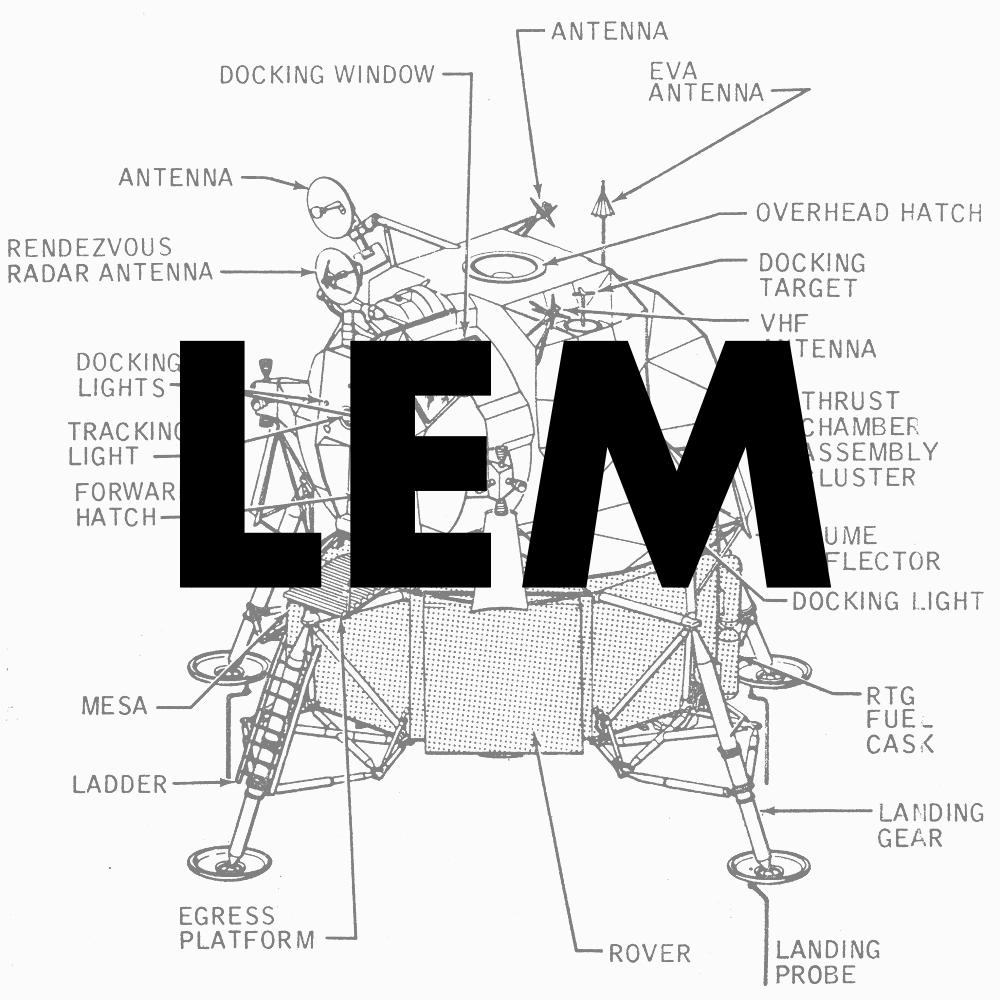
\includegraphics[width=1.25cm]{logo_LEM.png}% 27 Feb 2023
      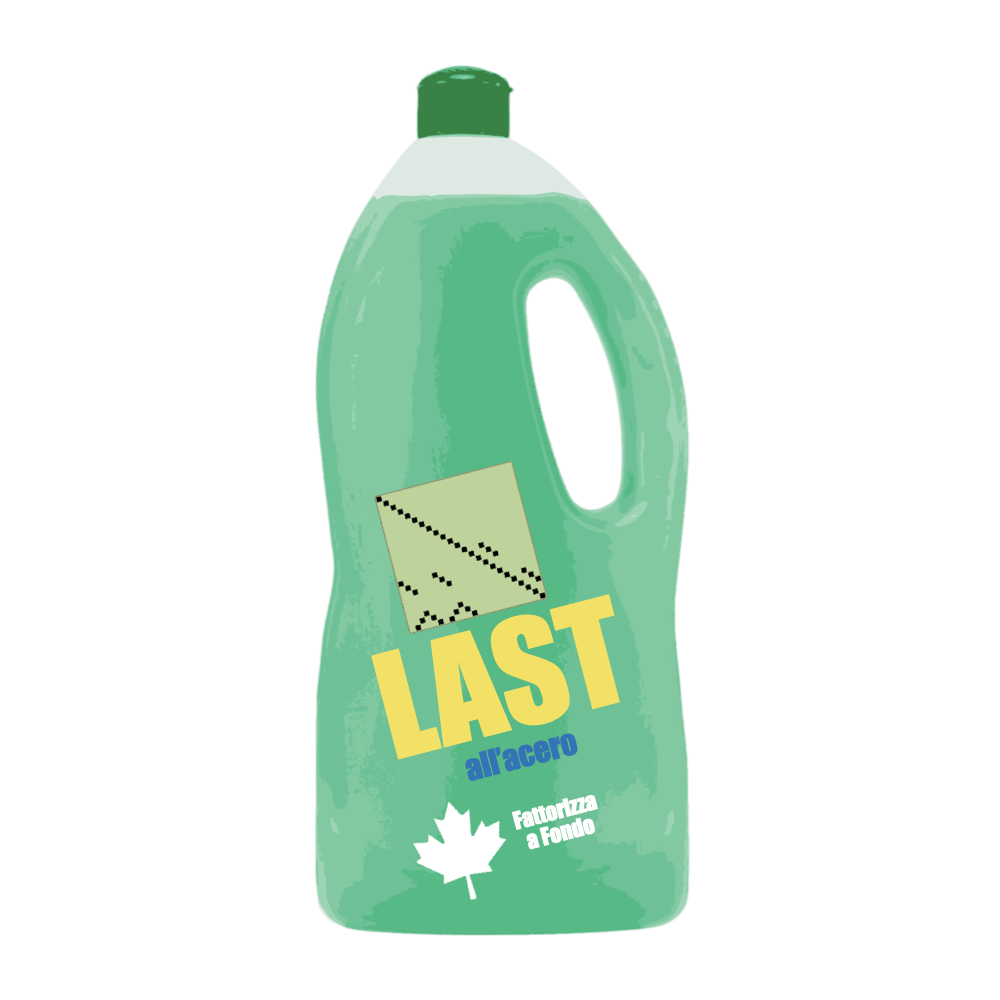
\includegraphics[width=1.25cm]{logo_LAST.png}% 28 Feb 2023
      
\includegraphics[width=1.25cm]{logo_Indigo.png}% 23 Jan 2023
      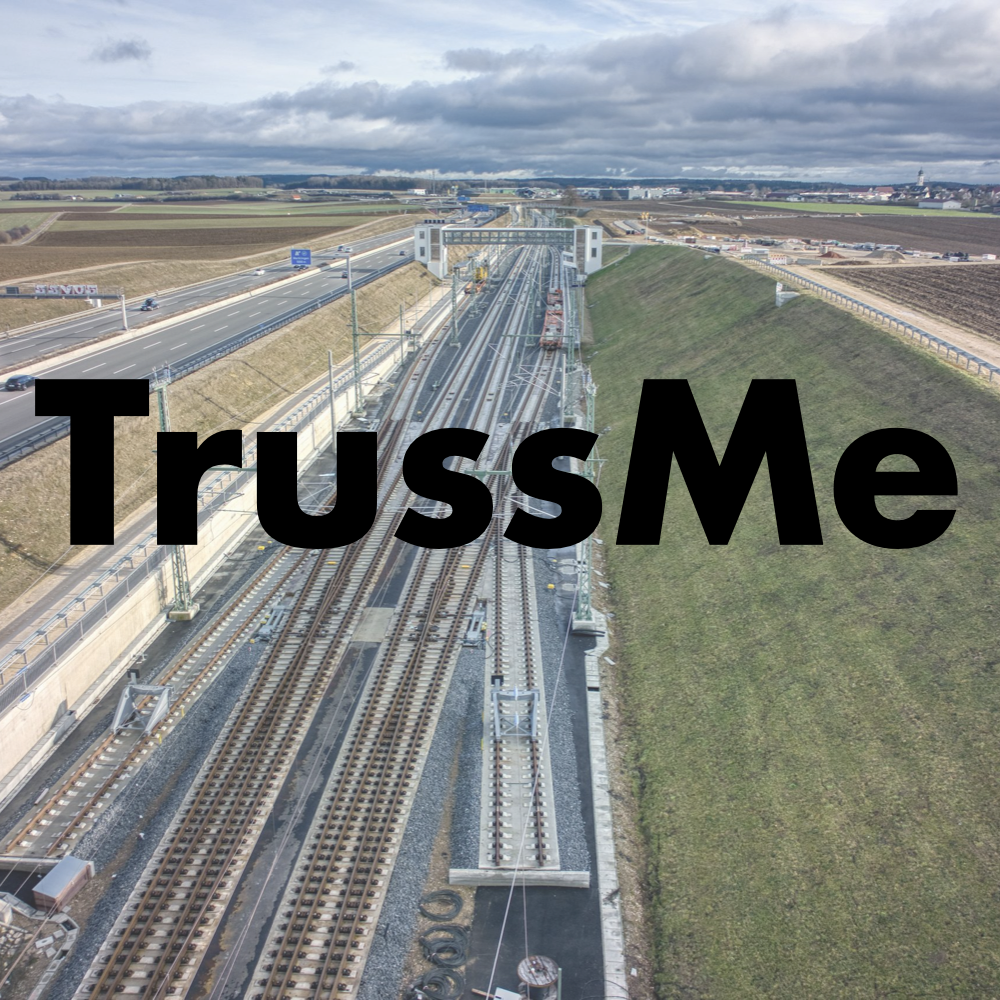
\includegraphics[width=1.25cm]{logo_TrussMe.png}%
      \includegraphics[width=1.25cm]{logo_TrussMe-FEM.png}% 25 May 2023
      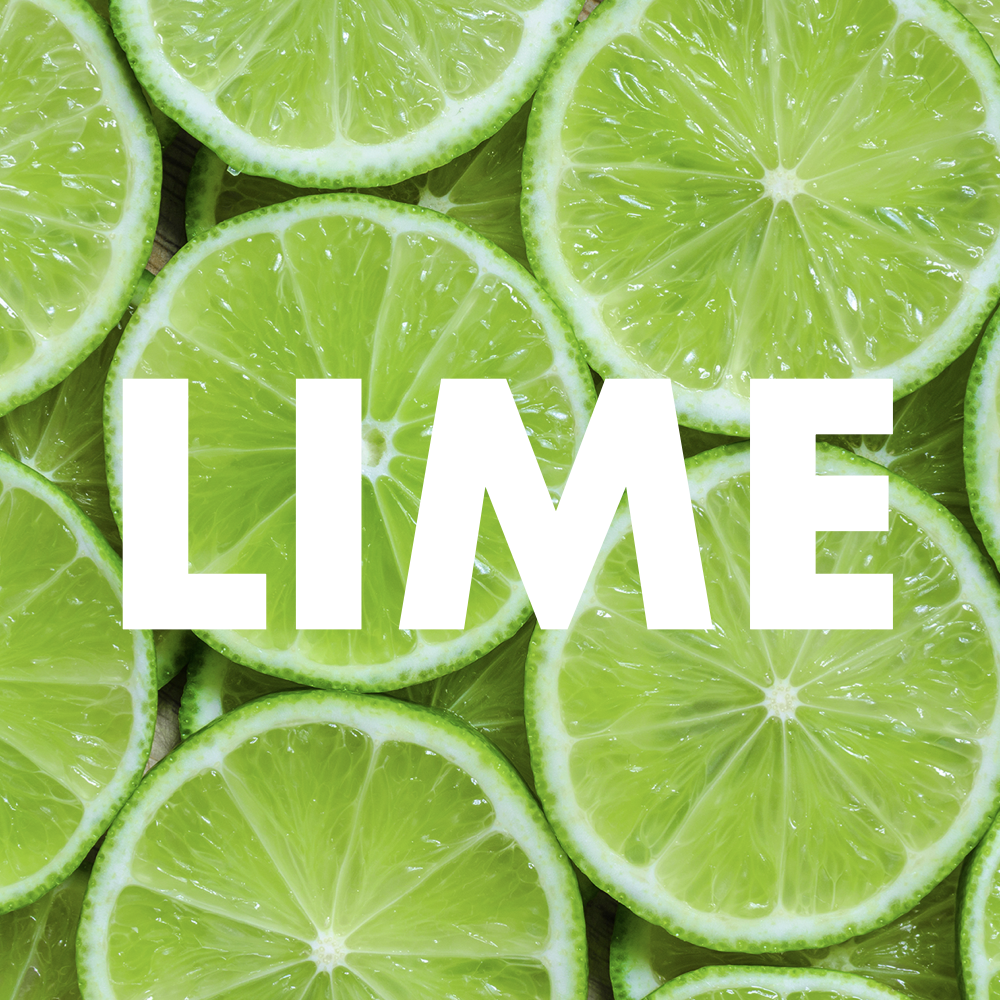
\includegraphics[width=1.25cm]{logo_Lime.png}%
      
\includegraphics[width=1.25cm]{logo_LimeRickey.png}
    \end{figure}
  \end{itemize}
\end{frame}

\begin{frame}{%
  Symbolic Computation Methods for the Numerical \\
  Solution of Dynamic Systems Described by \\
  Differential-Algebraic Equations
  }{Davide Stocco}
  \vfill
  \raggedright{\fontfamily{qag}\selectfont\Huge\color{tx_sl_color}\bfseries{Thank you for your attention!}} \\[0.5em]
  \raggedleft{\fontfamily{qag}\selectfont\Huge\color{tx_sl_color}\bfseries{Questions?}}
\end{frame}

% That's all Folks!